\documentclass[11pt,amsmath,amssymb]{article}

%\documentclass[twocolumn,amssymb,secnumarabic,preprintnumbers, %amsmath]{revtex4}
%\pdfoutput=1
%\documentclass[aps,10pt,twocolumn,showpacs,amsmath,amssymb,nofootinbib]{revtex4-1}

\usepackage{graphicx}
\usepackage{color}
\usepackage{soul}


%\pdfoutput=1 % if your are submitting a pdflatex (i.e. if you have
             % images in pdf, png or jpg format)

%\usepackage{jheppub} % for details on the use of the package, please
                     % see the JHEP-author-manual

\usepackage{longtable}
%\usepackage{widetable}
%\topmargin -1.5cm

\usepackage{graphicx}
%\usepackage{amssymb}
\usepackage{booktabs}
%\usepackage{color}
\usepackage{placeins}
\usepackage{multirow}
\usepackage{url}
%\usepackage{hyperref}

% \extracolsep{\fill}

\newcommand{\ra}[1]{\renewcommand{\arraystretch}{#1}}
\newcommand{\rb}[1]{\renewcommand{\tabcolsep}{#1}}

\usepackage{amsmath}
\usepackage{amssymb}

\newcommand{\C}[1]{{\cal C}_{#1}}
\newcommand{\B}{{\cal B}}

\newcommand{\ac}[1]{{\color{blue} #1}}

\newcommand{\ord}{\mathcal{O}}
\newcommand{\nn}{\noindent}
\newcommand{\nb}{\nonumber}
\newcommand{\arccot}{{\rm arccot}}
\newcommand{\sss}{\scriptscriptstyle}
\newcommand{\dis}{\displaystyle}
\newcommand{\eq}[1]{\begin{equation} #1 \end{equation}}
\newcommand{\eqa}[1]{\begin{eqnarray} #1 \end{eqnarray}}
\newcommand{\Cc}[1]{{\cal C}_{#1}}
\newcommand{\Cp}[1]{{\cal C}_{#1}'}
\newcommand{\delC}[1]{\delta {\cal C}_{#1}}
\newcommand{\dC}[1]{{\cal C}_{#1}^{\rm NP}}
\newcommand{\dCp}[1]{{\cal C}_{#1^\prime}^{\rm NP}}
\newcommand{\av}[1]{\langle #1 \rangle}
\newcommand{\afb}{A_{\rm FB}}
\newcommand{\red}[1]{{\color{red} #1}}
\newcommand{\qm}[1]{{\color{blue} #1}}
\newcommand{\jv}[1]{{\red {#1}}}

\newcommand{\sect}[1]{\section{\hspace{-0.3cm} #1}}

\begin{document}

\title{Report}
\author{Óliver Partida}
\date{\today}
\maketitle

\section{Data preprocessing}
Neural networks input are numbers which encode our data. The final goal of this step is to code our data using number that the  
\begin{itemize}
\item Drop irrelevant columns. Remove \textbf{ID} and \textbf{TIMESTAMP} columns from the training set. I believe these two fields are not relevant for the classification task. \textbf{TIMESTAMP} is the date the flight was booked and there are only two dates in the set.
\item Missing values. Remove from training and test data sets all rows that have columns with empty fields. The column \textbf{DEVICE} has several rows with empty values.
\item Transform dates to numerical value. The columns \textbf{DEPARTURE} and \textbf{ARRIVAL} have several different formats like \textbf{01/July} and \textbf{01-may} We have to transform the month name to its numerical value and remove the characters \textbf{-} and \textbf{/}.
\item Convert \textbf{DISTANCE} column to float. Replace \textbf{,} for \textbf{.}.

\item Encode categorical columns. For the columns \textbf{WEBSITE}, \textbf{DEVICE}, \textbf{HAUL TYPE}, \textbf{TRIP TYPE}, \textbf{PRODUCT} we use hot encoding. In this encoding each category is transformed into a new column. The category that any particular row had will be represented now by a 1 in the column assigned to that category and zeros in all the others. For the columns \textbf{SMS} and \textbf{TRAIN} we replace the values \textbf{TRUE/FALSE} with \textbf{1/0}.

\item Scale the data. We scale the columns \textbf{DISTANCE}, \textbf{DEPARTURE} and \textbf{ARRIVAL} to be in the range 0,1.  

\item Finally we transform the targets from \textbf{TRUE/FALSE} to \textbf{1/0}.
\end{itemize}
\section{Dimensionality reduction}
We have 82 features. In order to avoid the curse of dimensionality we attempt a principal component analysis to eliminate correlated features. In figure \ref{fig:Variance} we see that around 30 components suffice to explain most of the variance in the data.
\begin{figure}
	\centering
	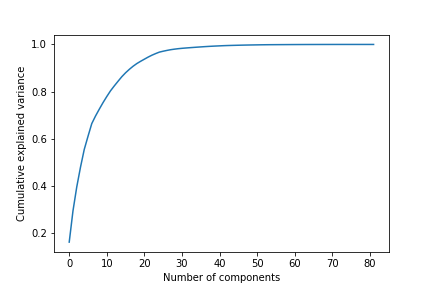
\includegraphics[width=0.8\columnwidth]{variance.png}
	\caption{Data variance explained by components}
	\label{fig:Variance}
\end{figure}
\section{NN training}
We tried a \textit{NN} with one input layer with 30 neurons, three hidden layers with 100, 50 and 20 neurons respectively and \textit{relu} activation function and finally an output layer with 1 neuron and \textit{sigmoid} activation function. The loss function is \textit{binary cross entropy}. The \textit{NN} is trained in 200 epochs with 2500 samples in each batch. In figures \ref{fig:accuracy} and \ref{fig:loss} we see the evolution of the NN accuracy and loss on the training set in blue and validation set in red. Although in the training set the accuracy increases and the loss decreases in the validation set the accuracy starts at some point to decrease and the loss to increase which means the algorithm is overfitting the data.
\begin{figure}
	\centering
	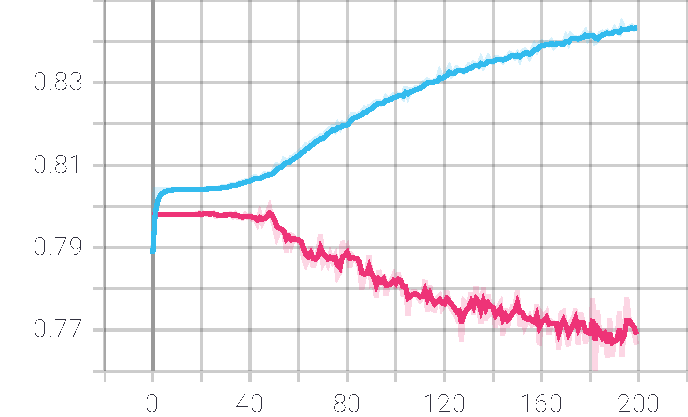
\includegraphics[width=0.8\columnwidth]{epoch_accuracy.pdf}
	\caption{Epoch accuracy}
	\label{fig:accuracy}
\end{figure}
\begin{figure}
	\centering
	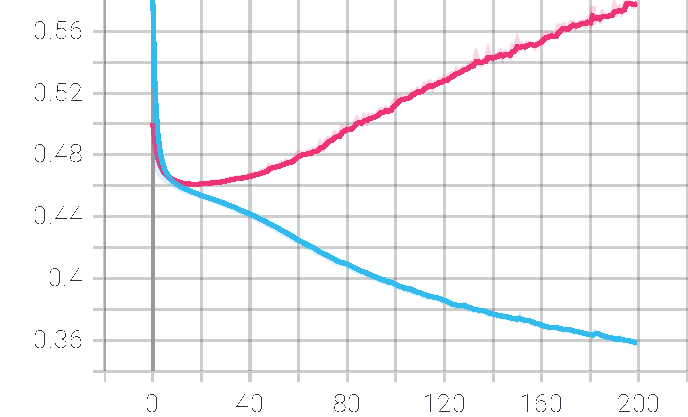
\includegraphics[width=0.8\columnwidth]{epoch_loss.pdf}
	\caption{Epoch loss}
	\label{fig:loss}
\end{figure}
\section{Conclusions}
Data preprocessing is a very important step to be able to train machine learning algorithms which can learn and extract patterns from the data. I did not have time to perform model selection to find the best NN architecture. The NN predicts 3162 samples that will buy extra baggage out of 30000 test samples. In 50000 samples in the training set there were 9799 samples that buy extra baggage. In we assume the test set have similar distribution the expected number of samples in the test set that would buy extra baggage is \(0.6\times 9799 = 5879 \). 
\end{document}
